%% This Beamer template is based on the one found here: https://github.com/sanhacheong/stanford-beamer-presentation, and edited to be used for Stanford ARM Lab

\documentclass[10pt]{beamer}
%\mode<presentation>{}

\usepackage{media9}
\usepackage{amssymb,amsmath,amsthm,enumerate}
\usepackage{mathtools}
\usepackage[utf8]{inputenc}
\usepackage{array}
\usepackage[parfill]{parskip}
\usepackage[utf8]{vietnam}
\usepackage{graphicx,animate}
\usepackage{caption}
\usepackage{subcaption}
\usepackage{bm}
\usepackage{amsfonts,amscd}
\usepackage[]{units}
\usepackage{listings}
\usepackage{multicol}
\usepackage{multirow}
\usepackage{tcolorbox}
\usepackage{physics}
\usepackage{movie15}
% Enable colored hyperlinks
\hypersetup{colorlinks=true}

% The following three lines are for crossmarks & checkmarks
\usepackage{pifont}% http://ctan.org/pkg/pifont
\newcommand{\cmark}{\ding{51}}%
\newcommand{\xmark}{\ding{55}}%

% Numbered captions of tables, pictures, etc.
\setbeamertemplate{caption}[numbered]
\usepackage{media9} 
%\usepackage[superscript,biblabel]{cite}
%\usepackage{algorithmic}
%\usepackage{algorithm2e}
%\usepackage{algpseudocode}
\usepackage[linesnumbered,ruled,vlined]{algorithm2e}
%\usepackage{algorithm}
%\usepackage{algorithmic}
\usepackage{caption}
%\usepackage{xcolor}
\usepackage{array}
%\renewcommand{\thealgocf}{}

\usepackage[natbib,backend=biber,style=ieee, sorting=ynt]{biblatex}
\bibliography{ref.bib}

\usepackage[acronym]{glossaries}

\usepackage{graphicx}
\graphicspath{{./figures}}
\usepackage{hyperref}

\theoremstyle{remark}
\newtheorem*{remark}{Remark}
\theoremstyle{definition}

%\newcommand{\empy}[1]{{\color{darkorange}\emph{#1}}}
%\newcommand{\empr}[1]{{\color{cardinalred}\emph{#1}}}
%\newcommand{\examplebox}[2]{
%\begin{tcolorbox}[colframe=darkcardinal,colback=boxgray,title=#1]
%#2
%\end{tcolorbox}}

%\usetheme{Stanford} 
%\def \i  {\item}
\def \ai {\item[] \quad \arrowbullet}
\newcommand \si[1]{\item[] \quad \bulletcolor{#1}}
\def \wi {\item[] \quad $\ \phantom{\Rightarrow}\ $}
\def \bi {\begin{itemize}\item}
\def \ei {\end{itemize}}
\def \be {\begin{equation*}}
\def \ee {\end{equation*}}
\def \bie {$\displaystyle{}
\def \eie {{\ }$}}
\def \bsie {\small$\displaystyle{}
\def \esie {{\ }$}\normalsize\selectfont}
\def \bse {\small\begin{equation*}}
\def \ese {\end{equation*}\normalsize}
\def \bfe {\footnotesize\begin{equation*}}
\def \efe {\end{equation*}\normalsize}
\renewcommand \le[1] {\\ \medskip \lefteqn{\hspace{1cm}#1} \medskip}
\def \bex {\begin{example}}
\def \eex {\end{example}}
\def \bfig {\begin{figure}}
\def \efig {\end{figure}}
\def \btheo {\begin{theorem}}
\def \etheo {\end{theorem}}
\def \bc {\begin{columns}}
\def \ec {\end{columns}}
\def \btab {\begin{tabbing}}
\def \etab {\end{tabbing}\svneg\svneg}
\newcommand \col[1]{\column{#1\linewidth}}
\def\vneg  {\vspace{-5mm}}
\def\lvneg {\vspace{-10mm}}
\def\svneg {\vspace{-2mm}}
\def\tvneg {\vspace{-1mm}}
\def\vpos  {\vspace{5mm}}
\def\lvpos {\vspace{10mm}}
\def\svpos {\vspace{2mm}}
\def\tvpos {\vspace{1mm}}
\def\hneg  {\hspace{-5mm}}
\def\lhneg {\hspace{-10mm}}
\def\shneg {\hspace{-2mm}}
\def\thneg {\hspace{-1mm}}
\def\hpos  {\hspace{5mm}}
\def\lhpos {\hspace{10mm}}
\def\shpos {\hspace{2mm}}

\usetheme{Copenhagen}
\usecolortheme{seahorse}
\logo{
\includegraphics[height=0.5in]{logos/HUS-name.jpg}}

\makeatletter
\let\@@magyar@captionfix\relax
\makeatother

\title[Trực quan hóa dữ liệu]{Trực quan hóa văn bản và tài liệu}

\AtBeginSection[]
{
    \begin{frame}
        \frametitle{Nội dung}
        \tableofcontents[currentsection, subsectionstyle=show/show/hide]
    \end{frame}
}

\setbeamertemplate{page number in head/foot}[totalframenumber]
\setbeamertemplate{frametitle continuation}{}

\begin{document}
\nocite{*}

\author[Nguyễn Chí Thanh - 21007925]{
	\begin{tabular}{c} 
	\Large
	Nguyễn Chí Thanh \\
    \footnotesize \href{mailto:nguyenchithanh\_sdh21@hus.edu.vn}{nguyenchithanh\_sdh21@hus.edu.vn}
\end{tabular}
\vspace{-4ex}}

\institute{
	\vskip 5pt
	\begin{figure}
		\centering
		\begin{subfigure}[t]{0.5\textwidth}
			\centering
			
\includegraphics[height=0.75in]{logos/HUS-logo.jpg}
		\end{subfigure}%
		~ 
		\begin{subfigure}[t]{0.5\textwidth}
			\centering
			
\includegraphics[height=0.75in]{logos/MIM-logo.png}
		\end{subfigure}
	\end{figure}
	\vskip 5pt	
	Đại học Quốc Gia Hà Nội \\
	Trường đại học Khoa học tự nhiên\\
	Khoa Toán - Cơ - Tin học
	\vskip 3pt
}

%\begin{noheadline}
\begin{frame} \maketitle \end{frame}
%\end{noheadline}
    
\setbeamertemplate{itemize items}[default]
\setbeamertemplate{itemize subitem}[circle]

\begin{frame}{Nội dung}
    \tableofcontents[hidesubsections]
\end{frame}

\section{Các cấp biểu diễn văn bản}

\subsection{Cấp độ từ vựng}

\begin{frame}{Cấp độ từ vựng}
	\begin{itemize}
		\item Cấp độ từ vựng liên qua đến việc biến đổi một chuỗi các ký tự sang một dãy các thực thể nguyên tử được gọi là \textit{tokens}.
		\item Bộ phân tích từ vựng xử lý dãy các ký tự với một bộ quy tắc nhất định thành một dãy các tokens mới có thể được sử dụng cho những phân tích sâu hơn.
		\item Tokens có thể bao gồm các ký tự, các ký tự n-grams, các từ, các gốc từ, các từ vựng, các cụm từ.
	\end{itemize}
    
\end{frame}

\subsection{Cấp độ cú pháp}

\begin{frame}{Cấp độ cú pháp}
	\begin{itemize}
		\item Cấp độ cú pháp liên quan đến việc xác định và gắn thẻ (chú thích) cho từng chức năng của tokens
		\item Quá trình trích xuất các gán nhãn này được gọi là \textit{nhận diện thực thể được đặt tên} (NER).
	\end{itemize}
\end{frame}

\subsection{Cấp độ ngữ nghĩa}

\begin{frame}{Cấp độ ngữ nghĩa}
	\begin{itemize}
		\item Cấp độ ngữ nghĩa bao gồm việc trích xuất xuất các ý nghĩa và quan hệ giữa các phần tri thức thu được từ các cấu trúc được xác định ở cấp độ cú pháp.
	\end{itemize}
\end{frame}

\section{Mô hình không gian vector}

\begin{frame}{Mô hình không gian vector}
	\begin{itemize}
		\item  Tính toán vectors các thuật ngữ hoặc các từ là một bước thiết yếu cho nhiều kỹ thuật trực quan hóa và phân tích tài liệu và văn bản.
		\item Trong \textit{mô hình không gian vector} \cite{356}, một vector của một thuật ngữ hoặc một từ cho một đối tượng quan tâm (đoạn văn, tài liệu hoặc một tập các tài liệu) là một vector mà trong đó mỗi chiều biểu diễn trọng số của một từ đã cho trong tài liệu đó.
		\item Thông thường, để loại bỏ nhiễu hoặc các từ dừng (stop words) (ví dụ "the", "a") được loại bỏ (lọc) và các từ có chung gốc được ghép vào làm một (ghép từ gốc).
	\end{itemize}
\end{frame}


\begin{frame}{Mô hình không gian vector}
	\begin{algorithm}[H]
        \DontPrintSemicolon
        $terms \gets \emptyset$\;
        \ForEach{$token$ $t$ \textbf{in} $tokenStream$}{
            \If{$t$ không phải là một từ dừng}{
                \If{$t$ \textbf{not in} $terms$} {
                    $terms \lbrack t \rbrack \gets 1$\;
                } 
                \Else {
                    $terms \lbrack t \rbrack \gets terms \lbrack t \rbrack + 1$\;
                }
            }
        }
        \Return{$terms$}\;
        \caption{COUNT-TERMS(tokenStream)}
        \label{alg:COUNT-TERMS}
    \end{algorithm}
\end{frame}

\begin{frame}{Mô hình không gian vector}
	\begin{table}[h!]
		\resizebox{10cm}{!}{%
        \begin{tabular} {|c| c| c| c| c| c| c| c| c| c|}
            \hline
            genetically & said & safety & engineered & study & test & great & deal & controversy & foods \\
            \hline
            3 & 3 & 2 & 2 & 2 & 2 & 1 & 1 & 1 & 1 \\
            \hline
        \end{tabular}
		}
    \end{table}
\end{frame}

\subsection{Tính toán các trọng số}

\begin{frame}{Tính toán các trọng số}
	\begin{itemize}
		\item Mô hình không gian vector yêu cầu một sơ đồ trọng số để gán trọng số cho các thuật ngữ ở trong một tài liệu.
		\item Có nhiều phương pháp để làm việc này, phương pháp nổi tiếng nhất trong số đó là tần số thuật ngữ - tần số tài liệu nghịch đảo (tf-idf) \cite{355}.
		\item  $Tf(w)$ là tần suất của thuật ngữ hay số lần mà từ $w$ xuất hiện trong tài liệu, và $Df(w)$ là tần suất của tài liệu (số tài liệu có chứa từ đó).
		Gọi $N$ là số tài liệu. Ta tính $TfIdf(w)$ theo công thức:
		\begin{equation}
			TfIdf(w) = Tf(w) \times \log \Big( \dfrac{N}{Df(w)} \Big)
		\end{equation}
	\end{itemize}
\end{frame}

\begin{frame}{Tính toán các trọng số}
	Mã giả ở thuật toán \ref{alg:COMPUTE-TFIDF} tính toán các vector tf-idf cho từng tài liệu.
	\resizebox{5cm}{!}{%
	\begin{algorithm}[H]
        \DontPrintSemicolon
        $termFrequencies \gets \emptyset$\; \tcp{Tra cứu bảng đếm số lần thuật ngữ/từ xuất hiện cho tên tài liệu}
        $documentFrequencies \gets  \emptyset$\; \tcp*{Đếm số tài liệu mà trong đó một thuật ngữ/từ nhất định xuất hiện}
        $uniqueTerms \gets \emptyset$\; \tcp*{Danh sách các thuật ngữ/từ riêng biệt}
        \ForEach{$document$ $d$ \textbf{in} $documents$}{
            $docName \gets NAME(d)$\; \tcp{Trích xuất tên của tài liệu}
            $tokenStream \gets TOKENIZE(d)$\; \tcp{Tạo luồng token của tài liệu}
            $terms \gets COUNT-TERMS(tokenStream)$\; \tcp{Đếm tần suất của các thuật ngữ/từ}
            $termFrequencies \lbrack docName \rbrack \gets terms$\; \tcp{Lưu trữ tần suất các thuật ngữ/từ tương ứng với từng tài liệu}
            \ForEach{$term$ $t$ \textbf{in} $KEYS(terms$)}{
                \If{$t$ \textbf{not in} $documentFrequencies$} {
                    $documentFrequencies \lbrack t \rbrack \gets 1$\;
                } 
                \Else {
                    $documentFrequencies \lbrack t \rbrack \gets documentFrequencies \lbrack t \rbrack + 1$\;
                }
                $uniqueTerms \gets uniqueTerms \cup t$\;
            }
        }
        $tfIdfVectorTable \gets \emptyset$\; \tcp{Tra cứu vector tf-idf cho tên tài liệu}
        $n \gets LENGTH(documents)$\;
        \ForEach{$document$ $name$ $docName$ \textbf{in} $KEYS(termFrequencies)$}{
            $tfIdfVector \gets $ \text{zeroes array of length} $LENGTH(uniqueTerms)$\;
            $terms \gets termFrequencies \lbrack docName \rbrack$\;
            \ForEach{$term$ $t$ \textbf{in} $KEYS(terms)$}{
                $tf \gets terms \lbrack t \rbrack$\;
                $df \gets documentFrequencies \lbrack t \rbrack$\;
                $tfIdf \gets tf \times \log \Big( \dfrac{n}{df} \Big)$\;
                $tfIdfVector \lbrack \text{chỉ số của } t \text{ trong } uniqueTerms \rbrack \gets tfIdf$\;
            }
            $tfIdfVectorTable \lbrack docName \rbrack \gets tfIdfVector$\;
        }
        \Return{$tfIdfVectorTable$}\;
        \caption{COMPUTE-TFIDF(documents)}
        \label{alg:COMPUTE-TFIDF}
    \end{algorithm}
	}
\end{frame}

\begin{frame}
	\begin{figure}[h!]
        \centering
        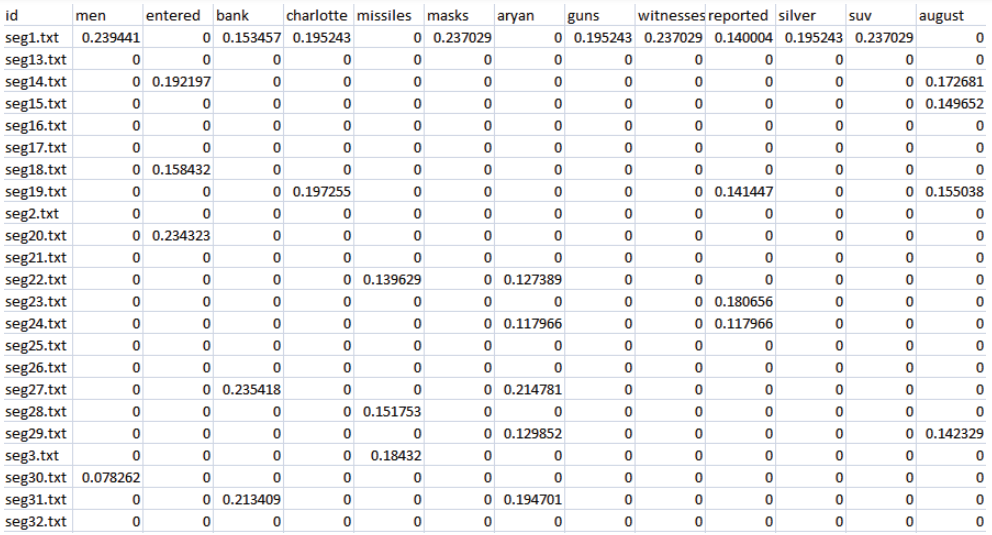
\includegraphics[width=0.8\textwidth]{1.png}
        \caption{Minh họa của các vector của các thuật ngữ trong nhiều tài liệu, bao gồm giá trị tf-idf.}
        \label{fig:1}
    \end{figure}
\end{frame}

\subsection{Định luật Zipf}

\begin{frame}{Định luật Zipf}
	\begin{itemize}
		\item Phân phối chuẩn và phân phối đều là các phân phối ta quen thuộc nhất.
		\item Phân phối hàm mũ ngày nay rất phổ biến với kích thước dữ liệu lớn, phản ánh hiện tượng mở rộng dữ liệu.
		\item Nhà kinh tế học Vilfredo Pareto tuyên bố rằng doanh thu của một công ty tỷ lệ nghịch với thứ hạng của công ty này, chính là tuân theo phân phối mũ kinh điển,
		dẫn đến quy tắc 80 - 20, trong đó 20\% dân số nắm giữ 80\% tài sản
	\end{itemize}
	
\end{frame}

\begin{frame}{Định luật Zipf}
	\begin{figure}[h!]
        \centering
        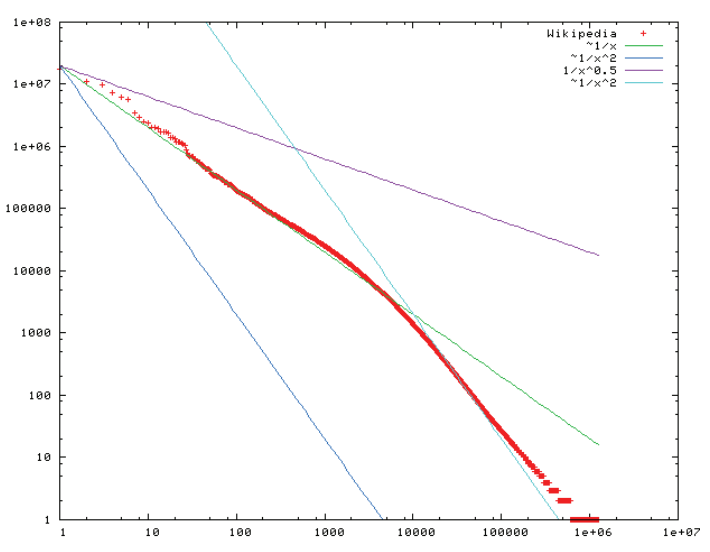
\includegraphics[width=0.8\textwidth]{2.png}
        \caption{Phân phối của các thuật ngữ trong Wikipedia, một ví dụ về luật Zipf.
        Phân phối của các thuật ngữ nằm trên trục y, và thứ hạng tần suất nằm trên trục x.}
        \label{fig:2}
    \end{figure}

\end{frame}

\begin{frame}{Định luật Zipf}
	\begin{itemize}
		\item Phân phối của các từ trong corpora tuân theo phân phối mũ được gọi là phân phối Zipf.
		\item Định luật Zipf \cite{490} phát biểu rằng trong một tài liệu ngôn ngữ tự nhiên điển hình, tần suất của một từ tỷ lệ nghịch với thứ hạng của nó trong bảng tần suất.
		\item Vẽ đồ thị đường cong Zipf trên thang đo log - log ta thu được một đường thẳng có hệ số góc -1 (hình \ref{fig:2}).
		\item Ý nghĩa của định luật Zipf là một lượng nhỏ các từ miêu tả hầu hết các khái niệm chính trong các tài liệu nhỏ.
	\end{itemize}
\end{frame}

\subsection{Các nhiệm vụ sử dụng mô hình không gian vector}

\begin{frame}{Các nhiệm vụ sử dụng mô hình không gian vector}
	\begin{itemize}
		\item Mô hình không gian vector, khi đi cùng với một độ đo khoảng cách cho phép ta thực hiện nhiều tác vụ hữu ích.
		\item Ta có thể sử dụng tf-idf và mô hình không gian vector để nhận diện các tài liệu cần được quan tâm đặc biệt.
		\item Ví dụ, mô hình không gian vector, với việc sử dụng một số độ đo khoảng cách, sẽ cho phép ta trả lời câu hỏi tài liệu nào giống với một tài liệu cụ thể cho trước.
		\item Làm thế nào để giúp người dùng hiểu được ý nghĩa của toàn bộ corpus.
		\item Biến đổi các tà liệu này thành các vector, sau đó thực thi các thuật toán dựa trên các nhiệm vụ đang được quan tâm (đo độ tương tự, tìm kiếm, phân cụm) và thực hiện trực quan hóa.
	\end{itemize}
\end{frame}

\section{Trực quan hóa tài liệu đơn}

\subsection{Đám mây từ (Wordcloud)}

\begin{frame}{Đám mây từ (Wordcloud)}
	\begin{figure}[h!]
        \centering
        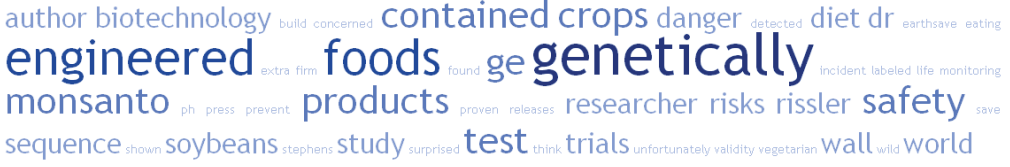
\includegraphics[width=0.8\textwidth]{4.png}
        \caption{Trực quan hóa đám mây thẻ được tạo bởi dịch vụ miễn phí tagCrowd.com \cite{396}.
        Cỡ chữ và độ tối tỷ lệ thuận với tuần suất xuất hiện của từ trong tài liệu}
        \label{fig:4}
    \end{figure}
\end{frame}


\begin{frame}{Đám mây từ (Wordcloud)}
	Đám mây từ (hình \ref{fig:4}), còn được gọi là đám mây văn bản hoặc đám mây thẻ, là bố của các các token mà được tô màu và định cỡ hiển thị theo tần suất xuất hiện của chúng trong một tài liệu.
\end{frame}

\subsection{WordTree}

\subsection{TextArc}

\subsection{Sơ đồ vòng cung (Arc Diagrams)}

\subsection{Dấu ấn văn học (Literature Fingerprinting)}

\section{Trực quan hóa tập tài liệu}

\subsection{Bản đồ tự tồ chức}

\subsection{Hình nền chủ đề}

\subsection{Thẻ tài liệu}

\section{Các kỹ thuật trực quan hóa văn bản mở rộng}

\subsection{Trực quan hóa phần mềm}

\subsection{Trực quan hóa kết quả truy vấn}

\subsection{Trực quan hóa tập tài liệu theo thời gian}

\subsection{Biểu diễn các mối quan hệ}

\section{Tài liệu tham khảo}
\begin{frame}[allowframebreaks]{Tài liệu tham khảo}
    \printbibliography
\end{frame}
\end{document}

